\documentclass{article}
\usepackage[document]{ragged2e}
\usepackage{enumitem}
\usepackage{amssymb}
\usepackage[spaces,hyphens]{url}
\usepackage{amsthm}
\usepackage{bbm}
\usepackage{multicol}
\usepackage{dsfont}
\usepackage{fullpage}
\usepackage{listings}
\usepackage{fancyhdr}
\usepackage{titlesec}
\usepackage{hyperref}
\usepackage{xcolor}
\usepackage{stmaryrd}
\usepackage{tikzpagenodes}
\usepackage[T1]{fontenc}
\usepackage[utf8]{inputenc}
\usepackage{CJKutf8}
\usepackage[english]{babel}
\usepackage{titlesec}
\usepackage{pgfplots}
\pgfplotsset{width=10cm,compat=1.9}
\usepgfplotslibrary{external} 
\usepackage{tikz,tkz-tab,amsmath}
\usetikzlibrary{arrows}
\graphicspath{ {./images/} }
\newcommand\E{e}
\newcommand\R{\mathbb{R}}
\newcommand\N{\mathbb{N}}
\newcommand\Z{\mathbb{Z}}
\newcommand\K{\mathbb{K}}
\newcommand\Q{\mathbb{Q}}
\newcommand\C{\mathbb{C}}
\newcommand\T{\mathcal{T}}
\usepackage[headsep=1cm, headheight=1cm]{geometry}
% !TeX spellcheck = en_GB 

\newcommand\dspst{\displaystyle}
\def\prop#1{\underline{\textbf{#1}}}

\def\changemargin#1#2{\list{}{\rightmargin#2\leftmargin#1}\item[]}
\let\endchangemargin=\endlist

%\titleformat{\part}[block]{\filcenter}{}(1em){}
\titleformat{\part}[block]{\Huge\bfseries\filcenter}{\partname{} \\ \thepart}{1em}{\huge}


%Defines emphasis color
\definecolor{rycolor}{RGB}{200,20,255}
\definecolor{note}{RGB}{100,100,100}
\definecolor{background}{RGB}{0,20,70}

%Defining a multi-line comment
\newcommand{\comment}[1]{}

\title{Programming and Algorithms Project \\ Exploring the artistic value of function spaces through fractals}
%{course by Olivier Guès}
\author{Christopher Mazzerbo}
\date{Last updated on \today}


\begin{document}

\lstset{ 
  backgroundcolor=\color{background},
  basicstyle=\footnotesize\color{white},
  breakatwhitespace=false,
  breaklines=true,
  captionpos=b,
  commentstyle=\color{green},
  extendedchars=true,
  frame=single,
  keepspaces=true,
  keywordstyle=\color{orange},
  language=Python,
  morekeywords={j,np,define,...},
  deletekeywords={round,file,in},
  numbers=left,
  numbersep=5pt,
  numberstyle=\tiny\color{white},
  rulecolor=\color{purple},
  showspaces=false,
  showstringspaces=false,
  showtabs=false,
  stepnumber=2,
  stringstyle=\color{yellow},
  tabsize=2,
  title=\lstname,
  literate={á}{{\'a}}1 {ã}{{\~a}}1 {é}{{\'e}}1 
}


\titlespacing{\subsubsection}{5mm}{0cm}{0cm}

%title

\fancypagestyle{plain}{
\fancyfoot{}
}
\pagestyle{plain}
\maketitle
\vspace{5mm}
\hrule
\pagebreak


%Edit header
\pagestyle{fancy}
\fancyhf{}
\fancyhfoffset[L]{1cm} % left extra length
\fancyhfoffset[R]{1cm} % right extra length
\rhead{Programming and Algorithms Project - fractal art}
\lhead{\bfseries Christopher Mazzerbo}
\fancyfoot{}
\fancyfoot[C]{\thepage}

\tableofcontents
\pagebreak


The purpose of this document is to provide some explanations about my Programming and Algorithms project, which generates fractals through the iteration of complex functions. \\
\vspace{5mm}
I'm aware the title isn't very informative but that's because a more accurate one would be too long, so I'll go over what it's really about in the first section of this document. \\
\vspace{2mm}
I'll split the rest into two main sections, which I'm naming \underline{Maths details} and \underline{Coding details} for lack of better titles. The former will explain how the code relates to Fatou and Julia sets, and how images can be obtained from the methods I present, but I've compiled more in-depth details in an external document for this. The latter will focus on some more algorithmic coding challenges I had to overcome in order to translate the mathematical complexity (in both the literal and maths sense) into images a viewer can interact with.


\section{Subject choice and design philosophy}

I chose this subject because I've been working on fractals, and more specifically Julia / Fatou sets in my own time for over a year now, and I've coded complex function iteration in multiple languages now, from a python-like Matlab script, to writing a pure fragment shader in GLSL (this one is available on my GitHub as \texttt{pyogl-shader-tester}). \\
\vspace{5mm}

During summer 2023, I had the opportunity of working in a Centuri lab for a training course, during which I became familiar with the \texttt{napari} package, and soon realised that I would use it for a Julia set related project as it allowed the visualisation of $N$-dimensional \texttt{numpy} arrays. \\
\vspace{5mm}

I wanted to try something new and actually make a semi-interactive Julia set generator that would display images as they generated, and through my newly discovered optimisations of colourings thanks to maths literature, I was able to get the generator working, and the focus of my project would then be to add user-friendly features. \\
\vspace{5mm}

\section{Maths details}

\subsection{Computational functions of \texttt{fractalize.py}}

In this file, some functions are unused by the main browser file as they usually don't give the user easy to visualise images, but I left them in for testing as I intend to implement options for these in later versions. These functions are : \\
\underline{Black \& White colouring} \texttt{bw\_coloring}, \underline{HLS Domain Colouring} \texttt{hls\_dc}, and their utility function \texttt{reduce}. \\
\vspace{5mm}

The other functions are designed around \texttt{julia\_from\_2D\_array}, which, as the name implies generates an image (shape given as an argument) from the $2D$ array representing a function. \\
The reason I use an \textit{array} to represent a function instead of anything else is because lambda functions are very difficult to randomize without constricting the function space to a specific subset, and the best idea I could come up with to leave the user some freedom was to implement series expansions. \\
\vspace{5mm}

Let $A \in \mathcal{M}_{2,n}(\R)$, $A = (a_{ij})_{\underset{1 \leq j \leq n}{1 \leq i \leq 2}}$. Then : \\
$$f(z) = \sum_{k=1}^n{(a_{1k}+i a_{2k})z^k} = \sum_{k=1}^n{a_k'z^k}$$
is the series expansion of order $n$, of a certain function. According to the function we want to emulate, we can just feed a series expansion to the function to get a decent approximation of the Fatou set image. Note that the Julia set itself is very different and not unique to a function \cite{Lev97}, though this won't be explored here. \\
\vspace{5mm}

I limit the space to $\lVert a_k' \rVert_{\infty} < 1$ with the supnorm metric, because the best-looking results tend to gravitate around series expansions whose terms have small moduli. This could be better optimised but doesn't seem to affect the generation of interesting results. \\
\vspace{2mm}
The images also generate around the origin, in $B(0,2)$, also for the supnorm metric (which results in square images). \\
\vspace{5mm}

\subsection{Computational solution}

The most famous, and common approach used to approximate images of these sets, that often yield pretty fractals, is to consider the iteration $f^n(B)$ where $B$ is the supnorm ball representing the image. \\
For explanations of why this is the case, please read the annex or read thoroughly explained definitions \cite{Sut14}. \\
\vspace{5mm}

The \underline{Julia set} appears somewhat by "completion" of the Fatou set, as the union of boundaries of the $F_i$ is precisely what constitutes the Julia set. \\
\vspace{5mm}
\textbf{It's far too unlikely, with our discretization of the complex plane with \texttt{numpy.ogrid}, to find a $z \in \mathcal{J}_f$. The way we can tell what shape it has is by differentiating the Fatou components through the process of iteration.} \\
\vspace{5mm}

For better-looking results, I opted to use the \textit{Normalized Iteration Count} algorithm \cite{Jon19}. The source of this method seems to be lost to a faulty link in \cite{Sil13}, but I thought I'd rather use a more generalised version of the modified Bernstein equations provided so that the generated images would seem less repetitive. \\
\vspace{2mm}
This method produces smoother results by keeping track of iteration counts rather than actual values of the iterates. \\
\pagebreak

\begin{multicols}{2}
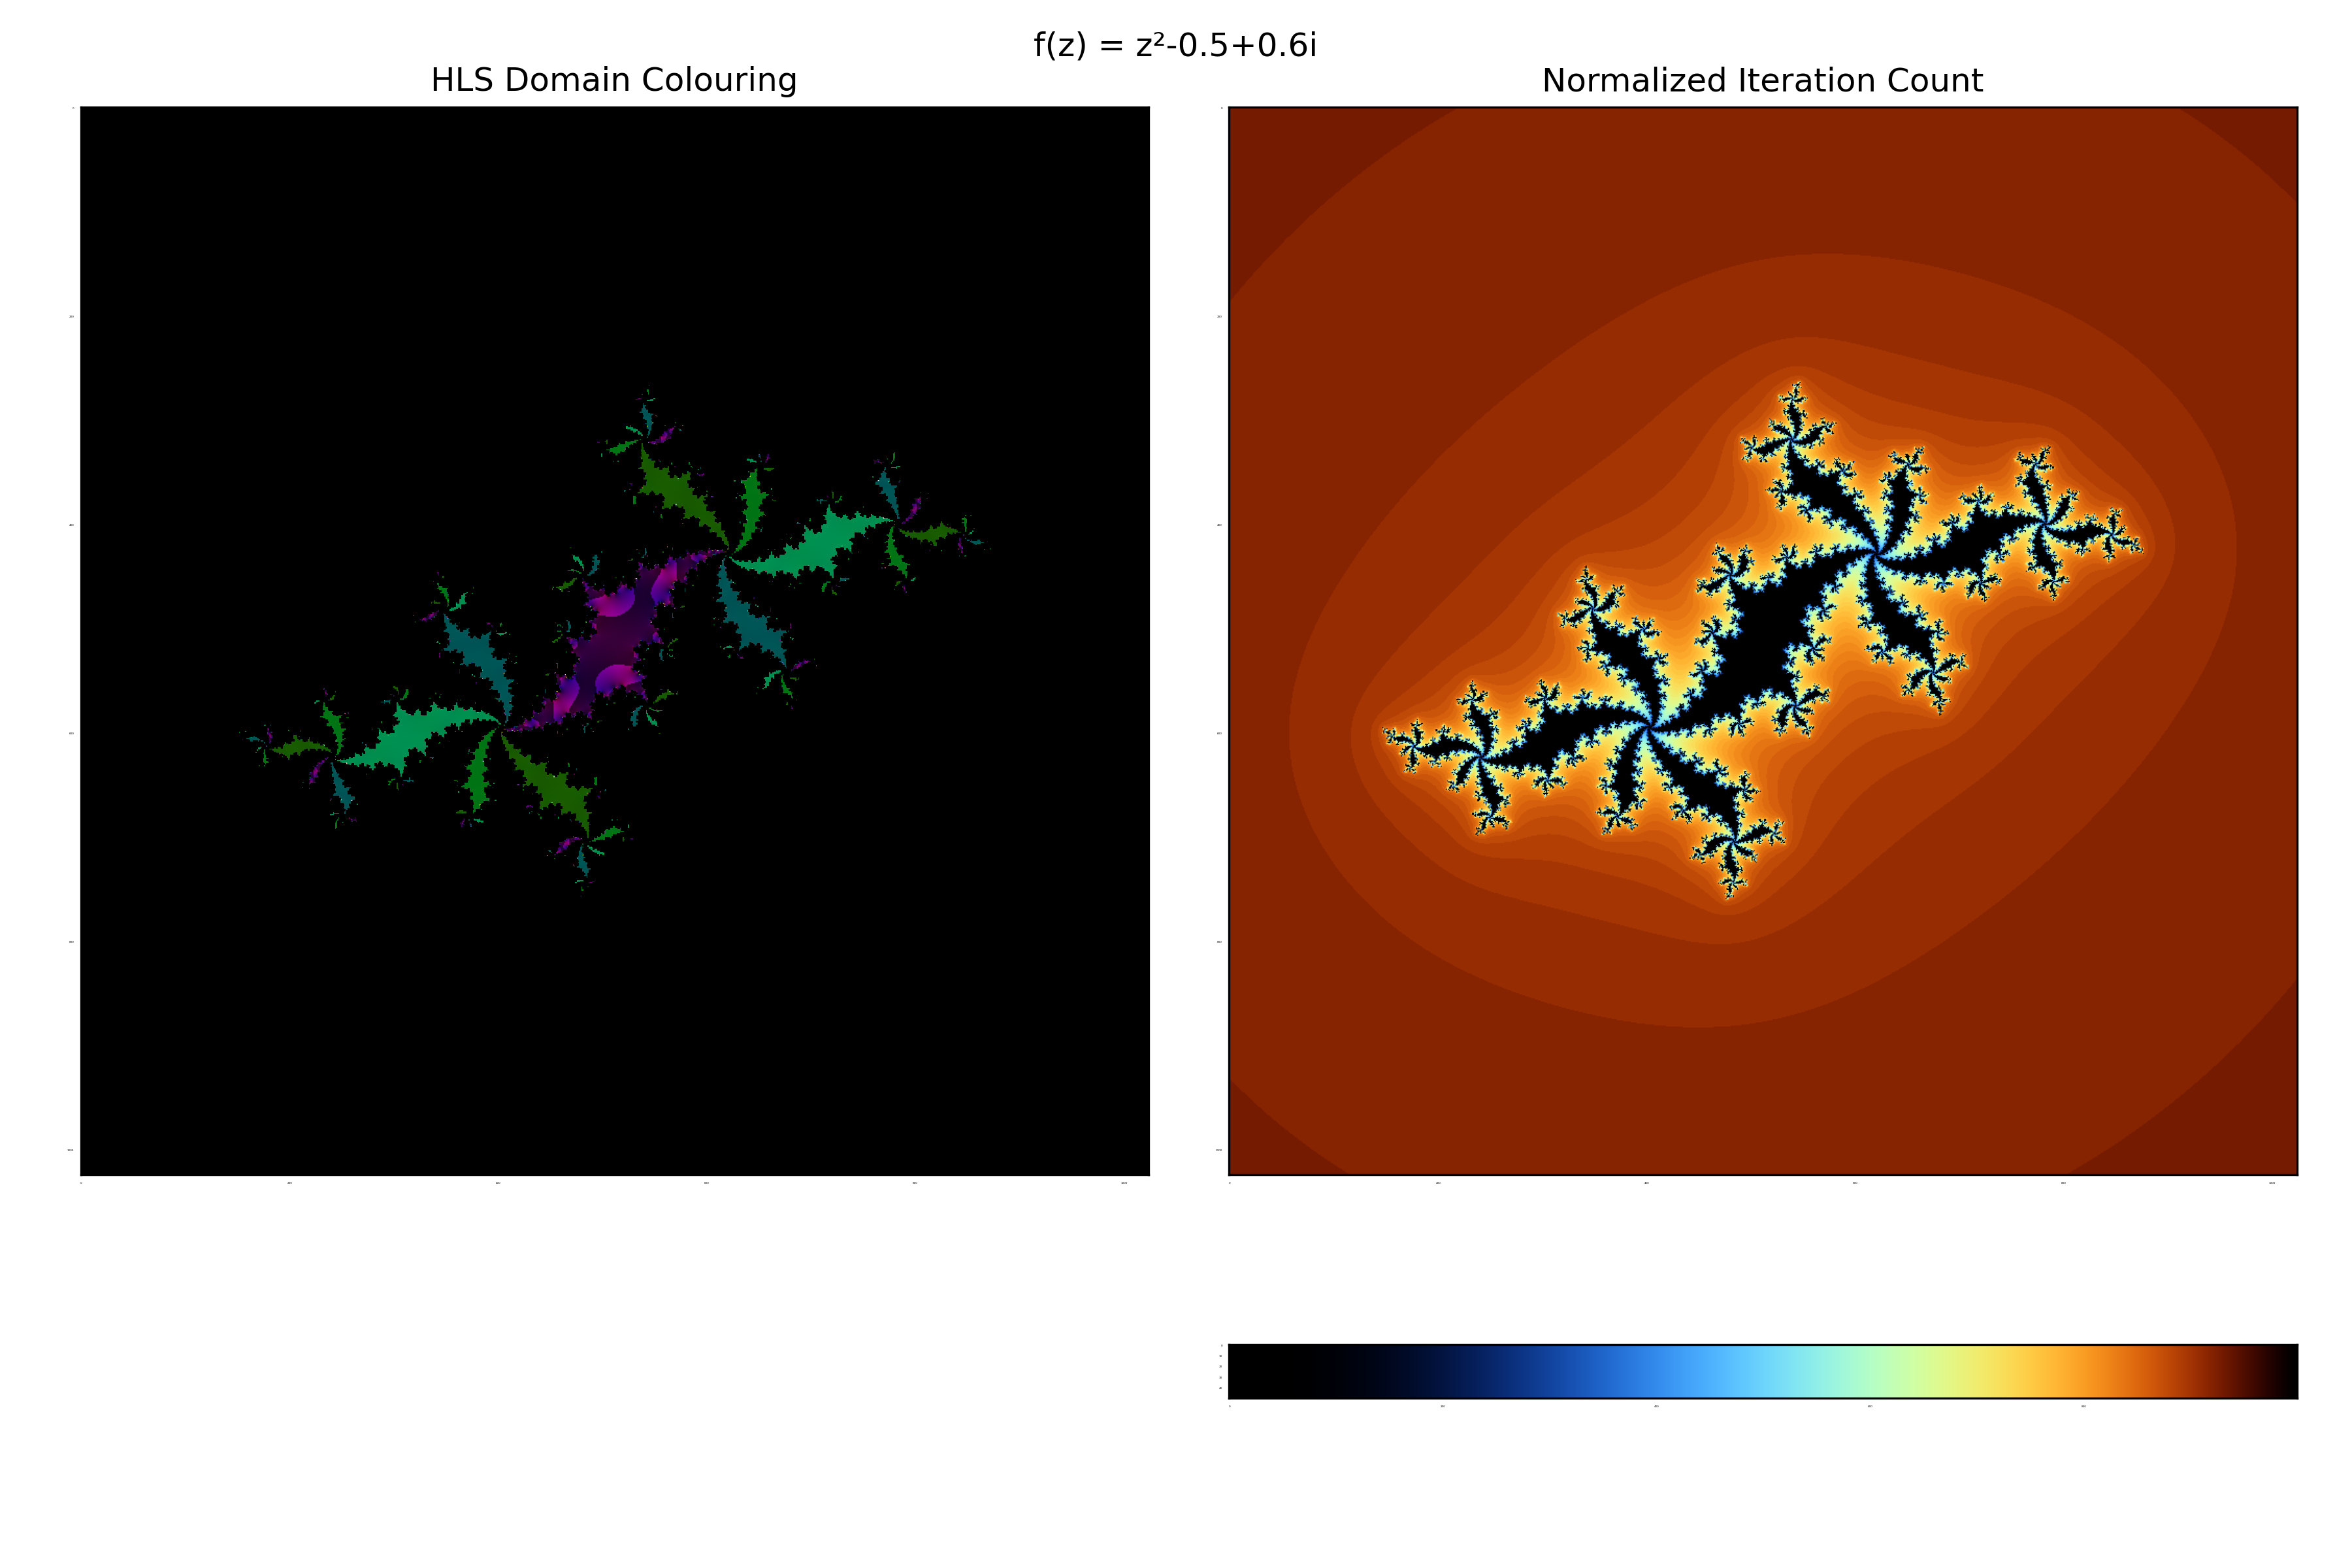
\includegraphics[scale=0.3]{hls_v_nic}
\columnbreak
\text{ } \\
\text{ } \\
\text{ } \\
\text{ } \\ %ugly asf but it works
\hspace{15mm}
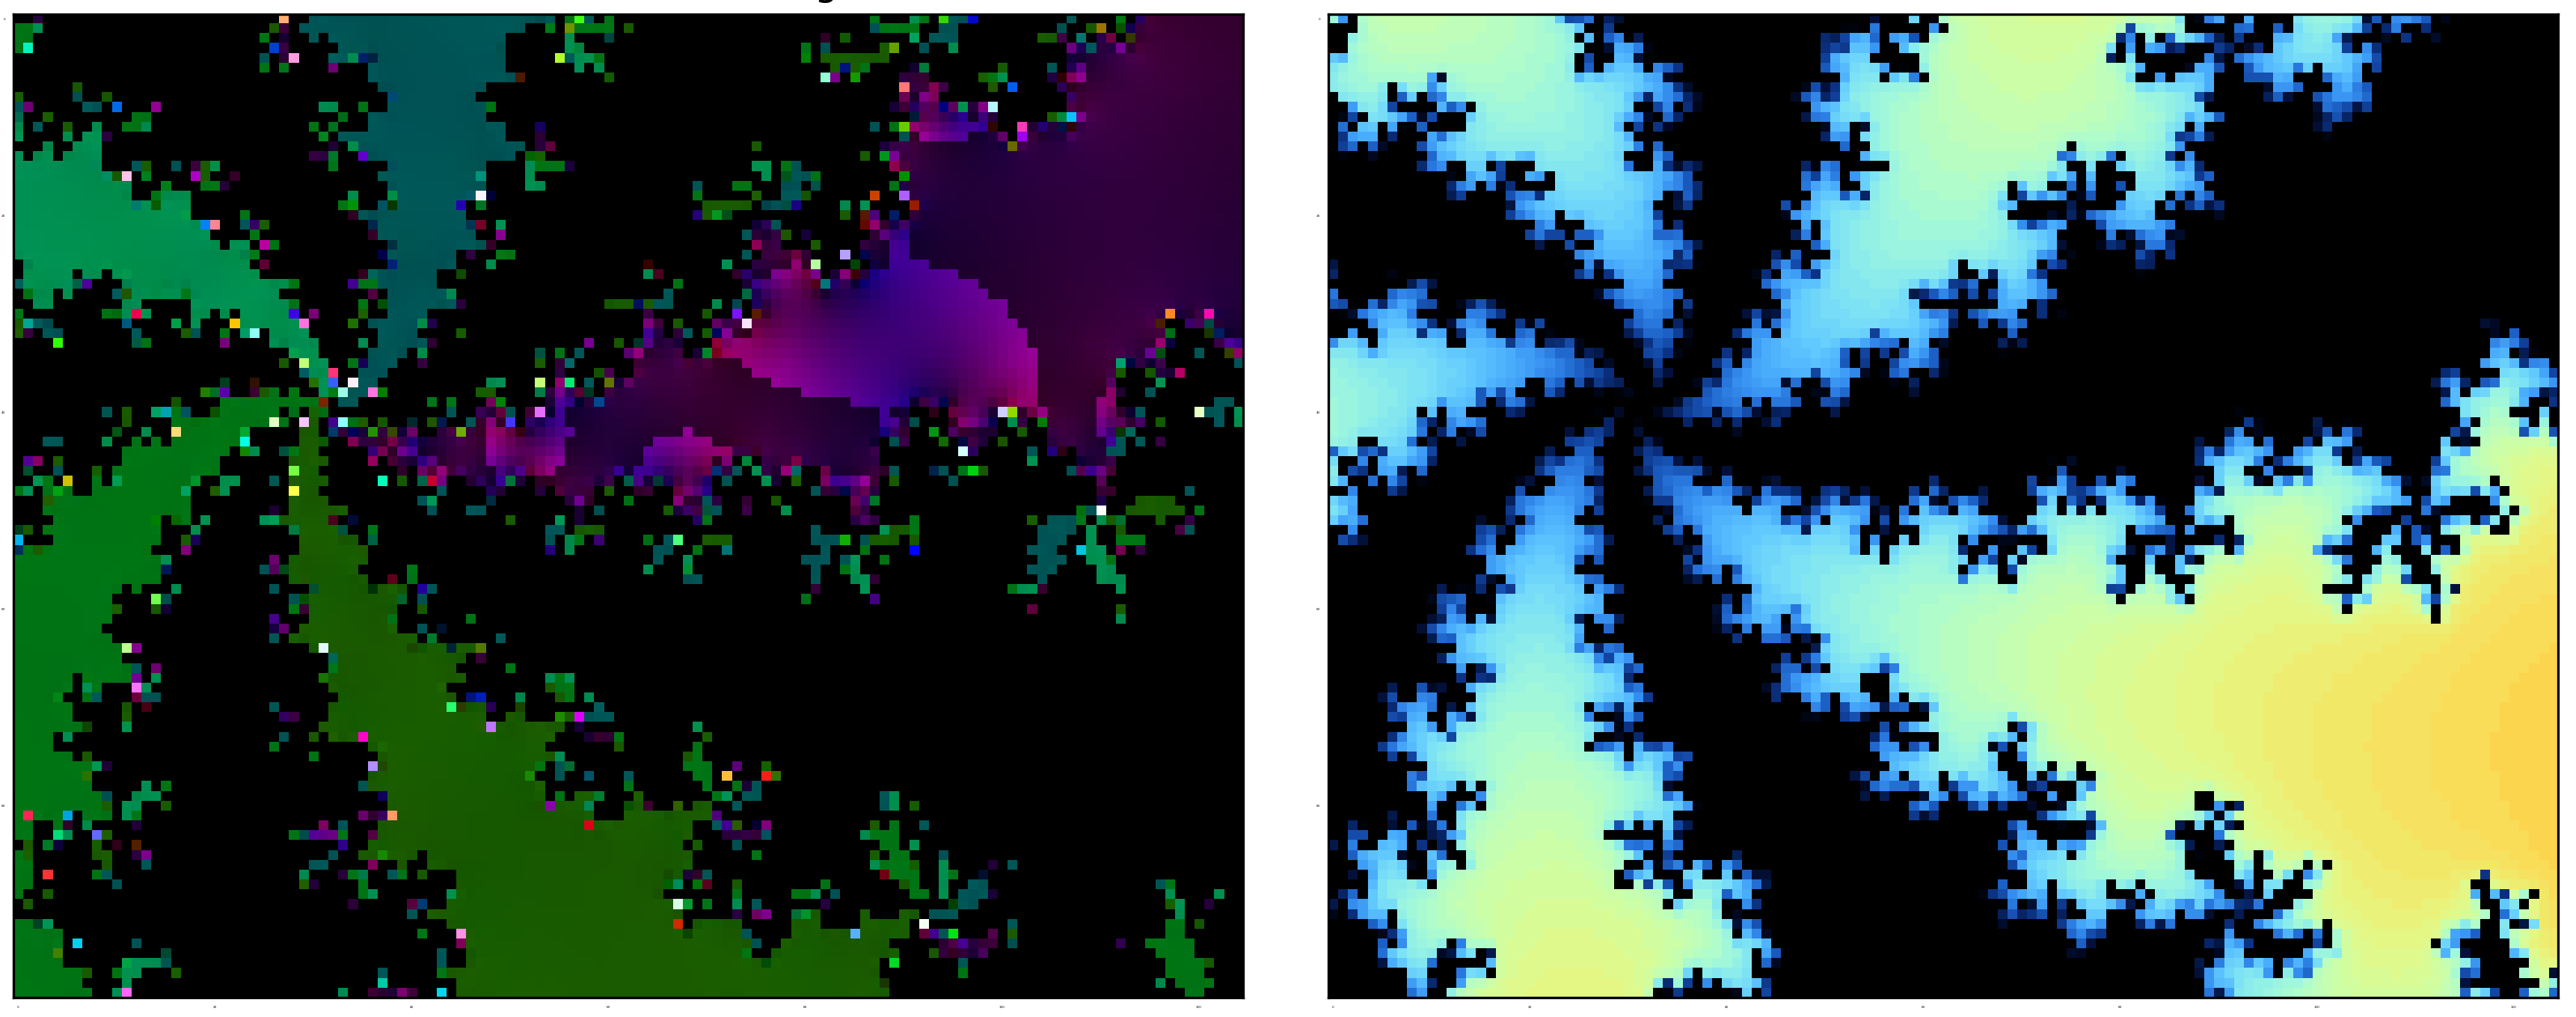
\includegraphics[scale=0.2]{hls_v_nic_zoom} \\
\end{multicols}
\vspace{-15mm}
\begin{center}
\textit{Display of banding differences between unused HLS domain colouring and Normalized Iteration Count}
\end{center}


Let's say we're computing $N$ iterations. Let $t_i := i/N$ where $0 \leq i \leq N$ is the $i$-th iteration. \\
To each pixel (represented by a $z \in \C$) on screen, we will assign the $t_i$ value corresponding to the first iteration where $\lvert f^{i}(z) \rvert$ goes over a certain upper limit (arbitrarily chosen at $10^{200}$ for better smoothness). \\
Then we apply the function $RGB : [0,1] \to [0,1]^3$ defined by : \\
$$RGB(t) = \begin{cases}
c_Rt^{l_R}(1-t)^{r_R} \\
c_Gt^{l_G}(1-t)^{r_G} \\
c_Bt^{l_B}(1-t)^{r_B}
\end{cases}$$
on all pixels of the image array. \\
\vspace{5mm}

$c_R$, $c_G$ and $c_B$ are constants that normalize the polynomials, so that the highest value of any component is always $1$. Normalising isn't strictly necessary, we only need the components to be less or equal to $1$. \\
\vspace{5mm}
$l_R$, $l_G$ and $l_B$ ($l$ for left), all strictly positive, are the multiplicities of the zero that appears at $t = 0$ for each component. Similarly, $r_R$, $r_G$ and $r_B$ are the multiplicities of the zeros that appear for $t = 1$. \\
Allowing those to vary can produce some very interesting colourmaps. \\
\vspace{5mm}

Most of the colourmaps generated this way share black colouring for $t = 0$ and $t = 1$, but as these correspond to parts of the set that are far away from each other it doesn't actually interfere with the quality of the image. \\
\vspace{5mm}

I integrated a "cmap analysis viewer" in the fractal browser so that the user could fully see how the colourmap affects the image. \\

\begin{center}
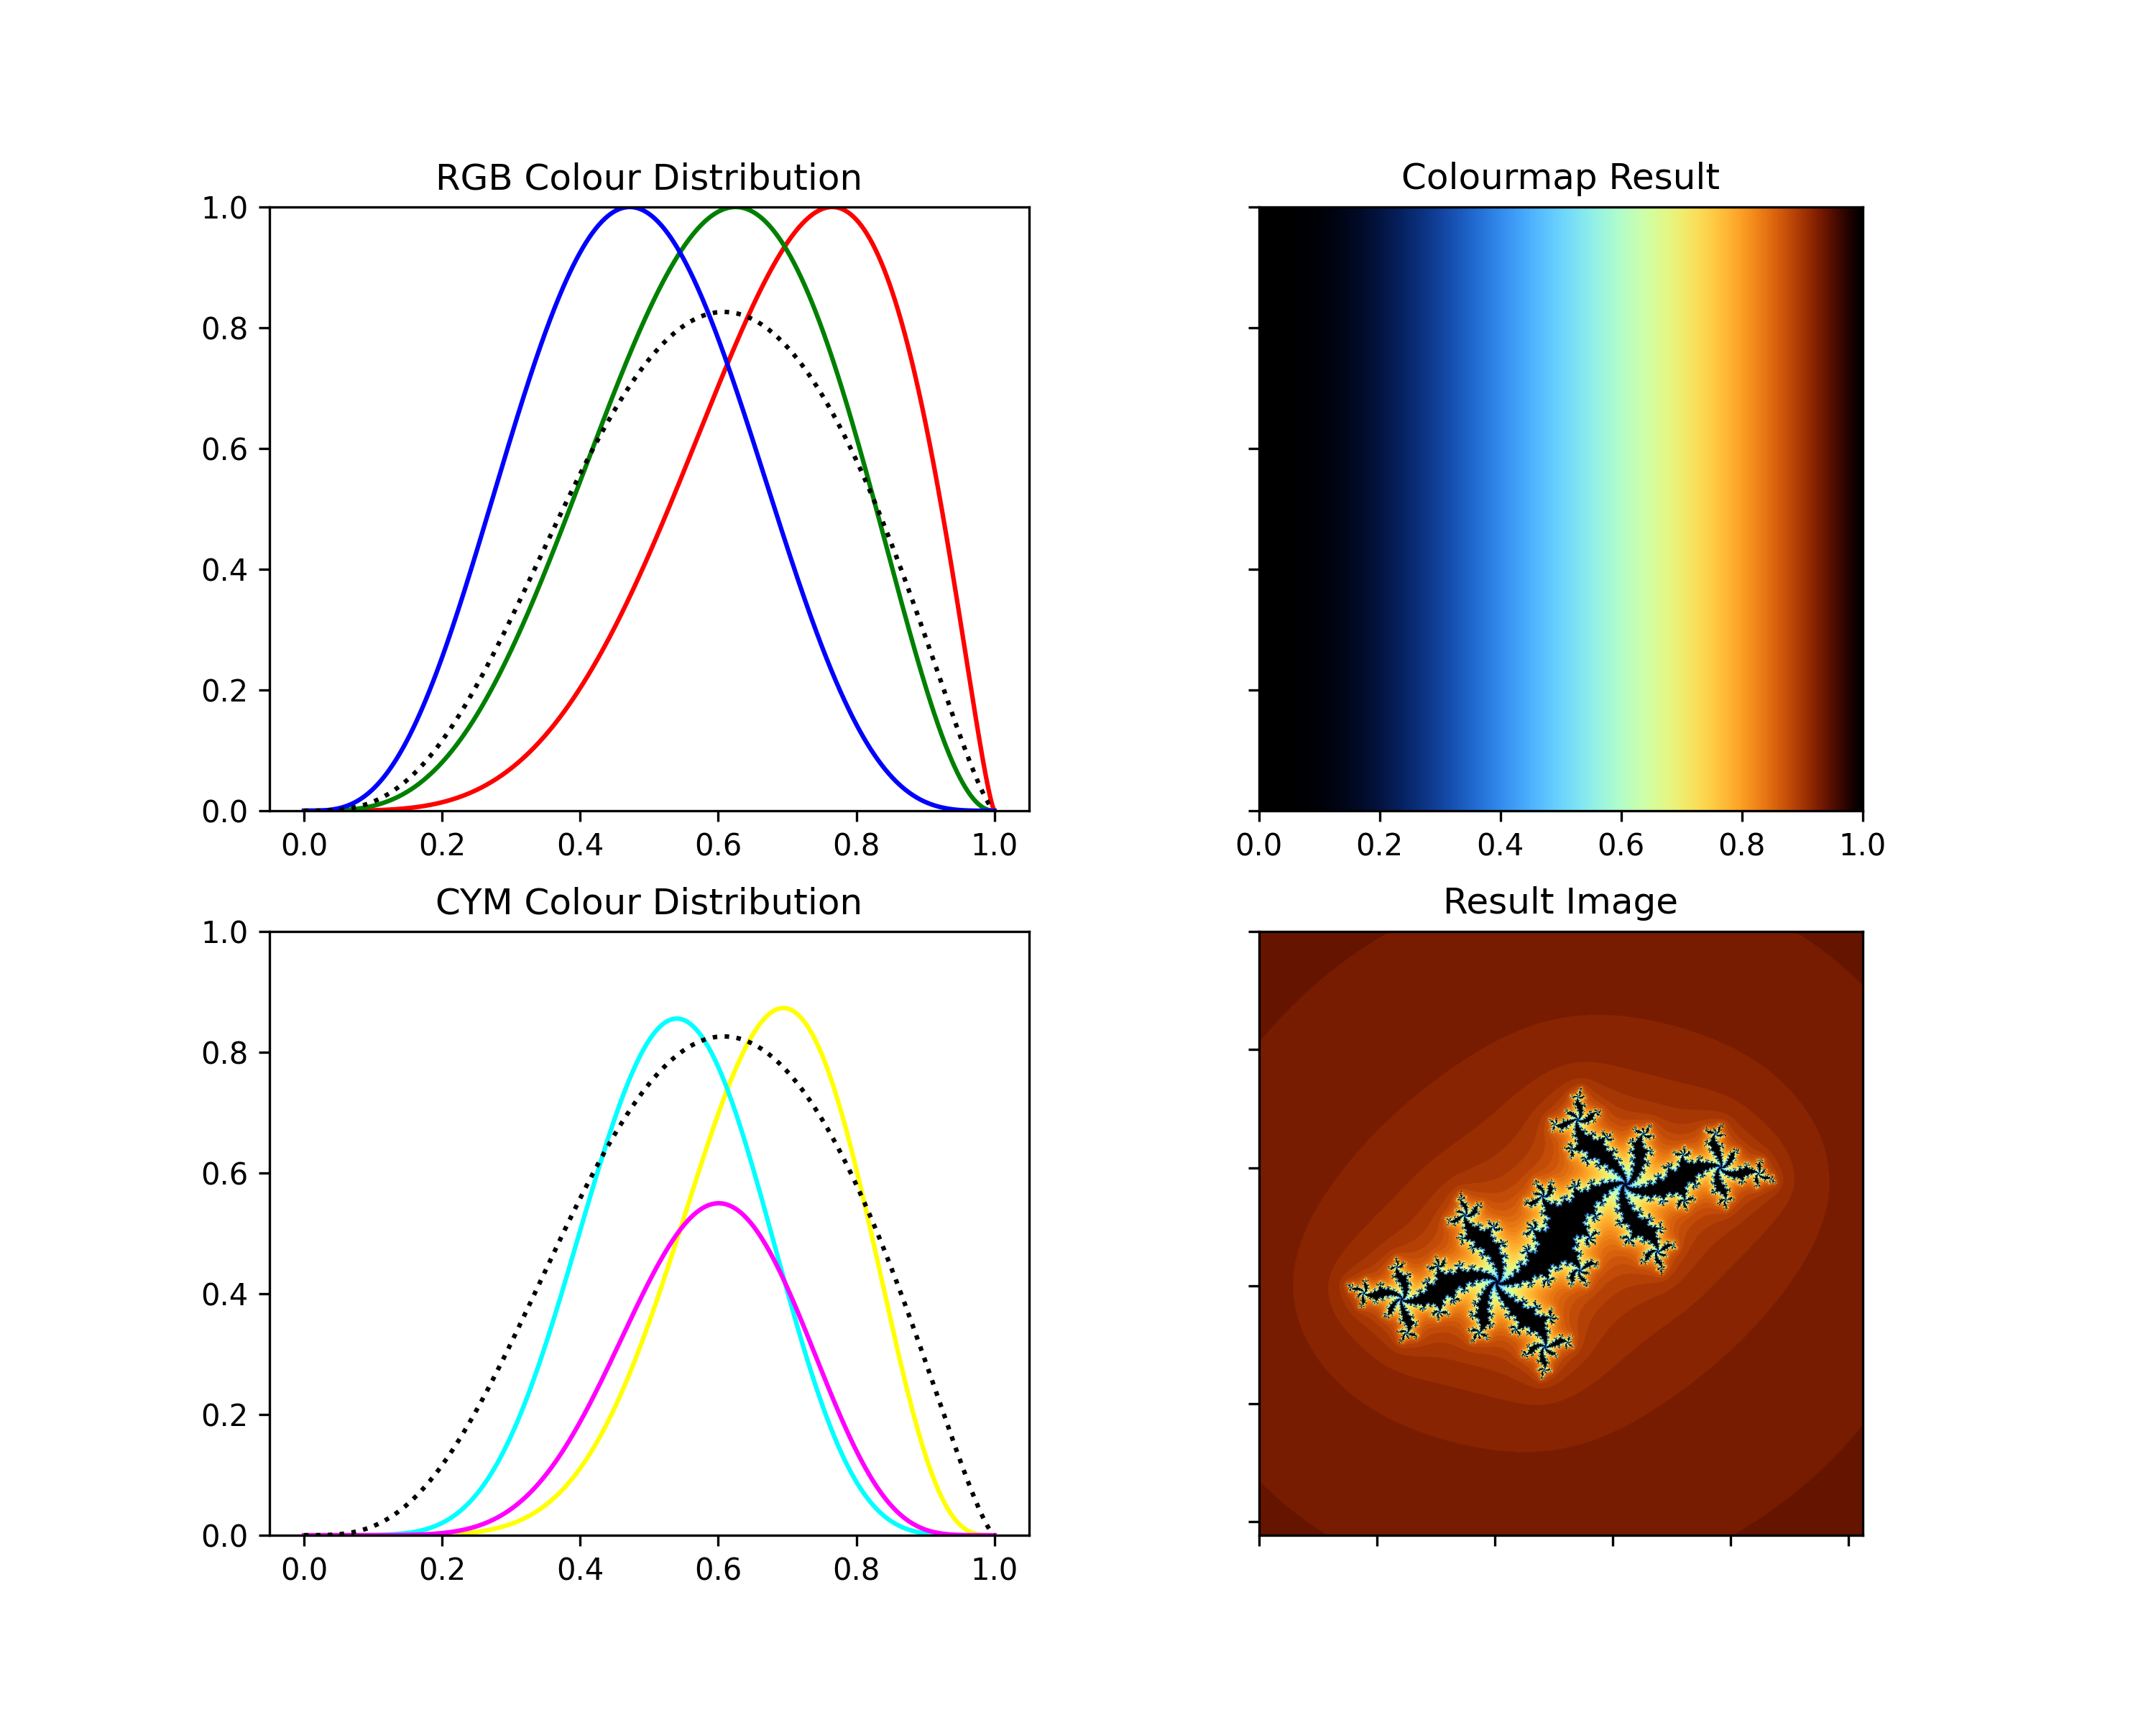
\includegraphics[scale=0.4]{report_params} \\
\textit{Additional data computed from a colourmap}
\end{center}


\section{Coding details}

\subsection{$N$-dimensional parametric spaces}

I have seen my fair share of fractal viewers online, but parametric spaces are rarely ever explored, which I've always found disappointing as it's known that the behaviour of $f^n(z)$ for certain $f$ can be very chaotic around certain points. \\
Most properties don't hold when taking limits, and as we are approximating Julia and Fatou sets through iteration, even the ones that do aren't trivial. \\
\vspace{5mm}

This thought brought me to the idea of displaying these images for $N$-dimensional parametric spaces of functions. \\
\vspace{5mm}

\subsubsection{Defining the linear interpolation}

Let $f, g$ be two functions defined by polynomials of order $k$. \\
I'll call $lerp$ the \textit{linear interpolation} of $f$ and $g$, that is : \\
\begin{equation}
\forall t \in \R, \quad lerp(t) = tf + (1-t)g
\end{equation}
The classical definition uses $t \in [0,1]$, but we can also use $t \in \R$, as for all $t \in \R$, $lerp(f,g)(t)$ is a function that is polynomial, and of order $k$. \\
\vspace{5mm}
By extending the definition of the lerp this way, we can say for these $f,g$, that $\dim \lbrace Span(lerp(f,g)(t)) \rbrace = \dim \lbrace t, t \in \R \rbrace = 1$. \\
In algebraic terms, $lerp(f,g) \in \mathcal{L}(\R, \mathcal{L}(\C, \C))$. \\
\vspace{5mm}

Now consider $L_1 = lerp(f_1,g_1)$, $L_2 = lerp(f_2,g_2)$. \\
As, for any $t \in \R$, $L_1(t)$ and $L_2(t)$ are complex polynomial functions of order $k$, we can define a new lerp : \\
$$\forall h \in \R, \quad lerp(L_1,L_2)(h) = hL1 + (1-h)L_2$$
or 
$$\forall (h,t) \in \R^2, \quad lerp(L_1,L_2)(h,t) = hL_1(t) + (1-h)L_2(t)$$
which of course yields $\dim \lbrace Span(lerp(L_1,L_2)(h,t)) \rbrace = 2$. \\
Note that $lerp(L_1,L_2) \in \mathcal{L}(\R, \mathcal{L}(\R, \mathcal{L}(\C, \C))) = \mathcal{L}^2(\R, \mathcal{L}(\C, \C))$. \\
\vspace{5mm}

\subsubsection{Generalisation and implementation}

We define the interpolated space as follows : \\

$$\forall p \geq 1, \quad \forall (F,G) \in \mathcal{L}^p(\R, \mathcal{L}(\C,\C))^2, \quad \forall t \in \R^{p+1}, \quad lerp(F,G)(t) = t_{p+1}F(t_0, \dots, t_p) + (1-t_{p+1})G(t_0, \dots, t_p)$$
Where of course if $p=0$ we can just use the traditional definition of a lerp given in $(1)$. \\
\vspace{5mm}

In reality, we only take $t \in [0,1]^{p+1}$, and as we can't \textit{actually} plot continuous spaces, I implemented a discrete version of this, with \texttt{lerp\_projector} and \texttt{fill}. Due to the nature of $lerp$, these are best defined as recursive functions. \\
\vspace{5mm}
I'll call a \texttt{(2,n)}-shaped array a \textit{function array} for convenience, as it represents a single function whose iterates will be computed. \\


\begin{lstlisting}[language=Python]
def lerp(arr1, arr2, size):
    return [arr1*(1-t) + arr2*t for t in np.linspace(0,1,size)]

def lerp_projector(space1, space2, size):
    if space1.shape != space2.shape:
        return
    if len(space1.shape) == 2:
        return np.array(lerp(space1, space2, size))
    space = []
    for a in range(len(space1)):
        arr1 = space1[a]
        arr2 = space2[a]
        space.append(lerp_projector(arr1, arr2, size))
    return np.array(space)
\end{lstlisting}

The function \texttt{lerp\_projector}, which takes two arrays of function arrays, of same shape (shape size $N$), returns a $N+1$ dimensional array containing the interpolated space of both arrays. \\
\vspace{5mm}
In this implementation, note that \texttt{lerp} is the version for $p=0$, and \texttt{lerp\_projector} is the generalised interpolation space function for all $p \geq 0$, which defaults to \texttt{lerp} if $p = 0$. \\
\vspace{5mm}
\begin{enumerate}[label=(\textit{\roman*})]
\item If $p = 0$, we are done. \\ 
\item If $p > 0$, then each element from one array is mapped to an element of the other array, which is always possible under the assumption that both arrays have identical shape. \\
These elements are by definition of dimension $p-1$ and of same shape, so passing them back through the \texttt{lerp\_projector} function is valid, and we return to (\textit{i}).
\end{enumerate}
This process ends and we end up retrieving an $(N+1)$-dimensional array of what I'm calling here the \textit{interpolated space} of function arrays. \\
\vspace{5mm}

\begin{lstlisting}
def fill(arr_list, new_resolution, ordertxt, progress_bar):
    dims = arr_list.shape[:-2]
    hyperplane = []
    if len(dims) > 1:
        for dim in range(dims[0]):
            hyperplane.append(fill(arr_list[dim,], new_resolution, ordertxt, progress_bar))
    else:
        for arr in arr_list:
            progress_bar.update(1)
            img = frctl.julia_from_2Darray(arr, (new_resolution,new_resolution), frctl.parametric_cmap)
            img = colorswap(img, ordertxt)
            img = (255*img).astype(np.uint8)
            hyperplane.append(img)
    return np.array(hyperplane)
\end{lstlisting}

The function \texttt{fill} takes as argument the $N$-dimensional interpolated space of desired functions, and generates the Julia/Fatou set images for every single image in that space. \\
The word \textit{image} here is used literally, in two dimensions, which means the a $1$-dimensional interpolated space ($lerp(f,g)$ for two functions $f,g$) would result in a $3D$ image. Obviously this becomes hard to visualise very quickly. \\
\vspace{2mm}
Luckily, \texttt{napari} is built for this type of data so we can use sliders to move around in the new space (there's even a 3D viewer already embedded in the software). \\
\vspace{5mm}

\begin{enumerate}[label=(\textit{\Roman*})]
\item If \texttt{len(dims)} is $1$, then it means the function has to "fill in" a $1D$ lerp of functions, so we can loop over all the function arrays in the lerp and compute the fractal image, adding it to a list called \texttt{hyperplane} which will later be returned. I call this the "hyperplane" because its shape is one dimension higher than the objects it is using (single function arrays). \\
\item If \texttt{len(dims)} is greater than $1$, then we iterate over the arrays through the first dimension, and return the filled in space of each of these. This leads us back to (\textit{I}).
\end{enumerate}

Again, the process ends as the returned \texttt{hyperplane} arrays are a dimension lower than the array list, meaning their shape size decrements by $1$. \\
\vspace{5mm}
I won't be including images of the results of this process as many of these can be accessed on the project's main page.


\subsection{Extra features}

Other features include : \\
\begin{itemize}
\item Loading an image array from an \texttt{.npy} array (shaped \texttt{(2,n)}) or \texttt{.frctl} file. \\
If the file is an \texttt{.npy} file, it uses current settings to compute the image.
\item Enhancing an existing image to a new resolution (can be lower or higher). \\
\item Setting global parameters (including colourmap parametric functions, using the console, but this is more advanced so not presented in the UI). 
\end{itemize}

\subsubsection{Shortcuts and misc}

Existing NumPad shortcuts for certain buttons are hardcoded using \texttt{napari}'s \texttt{bind\_key} decorator. These are indicated in parentheses in the buttons' call text : \\
\begin{itemize}
\item \texttt{0} adds a new random image. \\
\item \texttt{1} saves the image as a \texttt{.frctl} file in the current save folder. \\
\item \texttt{2} attempts to save a \texttt{.gif} file of a $1D$ lerp. This obviously fails if the image is not of the right shape \texttt{(k,RES,RES)}. \\
\item \texttt{3} deletes everything currently in the viewer. Global variables are conserved. \\
\item \texttt{r} isn't a NumPad shortcut, but randomizes the colourmap parametric functions using the general formula given in section 2.2.
\end{itemize}

In the napari console (default shortcut access through \texttt{Ctrl+Shift+C}), it's possible to modify the custom \texttt{viewer.layers[-1].metadata} dictionary to set custom parametric colourmap functions. \\
For example, we could set all of them to 
$$\forall t \in [0,1], \quad c(t) = 1-t$$
using : \\
\begin{lstlisting}
[viewer.layers[-1].metadata[f] = lambda t : 1-t for f in ("param_R","param_G","param_B")]
\end{lstlisting}
\vspace{-5mm}
for pure black and white images (specifically where $Bas(z)$ appears white regardless of $z \in \C$ and $Bas(\infty)$ appears black, see \cite{Sut14} section 3 for details). \\
\vspace{5mm}

For more variety in colourings for any given triplet of parametric functions, I decided to shuffle the red, green and blue functions randomly on image generation. \\
\vspace{2mm}
For image $i$ in the viewer, this order is stored in metadata as \texttt{viewer.layers[i].metadata["ordertxt"]} and appears as a reshuffle of the characters \texttt{"r"}, \texttt{"g"} and \texttt{"b"}. \\
\vspace{2mm}
This can be fixed using a size-1 lerp of the image with itself and setting the desired order in the lerp settings (of course, don't forget to set the resolution also). \\
\vspace{2mm}
Note that it's possible to set the \texttt{ordertxt} with repeats (so \texttt{"rrr"} would always give a black and white image for example).










\bibliographystyle{alpha.bst}
\bibliography{frctl_refs.bib}

\end{document}